\chapter{\sc PLEASE: The \textbf{P}ython \textbf{L}ow-energy \textbf{E}lectron \textbf{A}nalysis \textbf{S}uit\textbf{E}}
\newcommand{\shellcmd}[1]{\\\indent\indent\texttt{\footnotesize\# #1}\\}
\label{app:Appendix A PLEASE: Python Low-energy Electron Analysis SuitE}

% --- Insert Text --- %

\section{Introduction}
PLEASE is a software package written in python providing an open source fully cross-platform multithreaded graphical user interface (GUI) for data analysis of LEEM and LEED experiments with a specific emphasis on analysis of Intensity-Energy( \textit{I(V)} ) data sets. The software uses the Qt (pronounced 'cute') C/C++ application framework via the python bindings provided by the PyQt and PyQtGraph libraries. The software is hosted on GitHub and available for download at \url{https://www.github.com/mgrady3/PLEASE}. PLEASE is licensed under the GPL v. 3 software license provided within the source repository.

\section{Background and Motivation: Why is it?}
 Low energy electron microscopy and the associated technique of micro spot sized low energy electron diffraction are powerful tools for a wide variety of surface science experiments applicable to the study of various novel materials. Considering that many novel two-dimensional materials can currently only be easily synthesized as small flakes of single or few layer thickness and small lateral area, this form factor makes many surface science techniques ill-equipped for their analysis. LEEM and $\mu$-LEED are uniquely suited for the structural analysis of 2D materials through analysis of electron \textit{I(V)} data.

 After completing my initial LEEM investigation of the polymorphic graphene system at the Sandia National Laboratory's Center for Integrated Nano Technology, I was left with multiple Gb's of experimental data with no easy ``off the shelf'' method for performing the required analysis. At the time of the initial development of the PLEASE software package, there were no open source software packages to aid in the analysis of both LEEM and LEED data. There was one open source package for analysis of conventional LEED \textit{I(V)} data - EasyLEED - written by Andreas Mayer, however this program was not suited for the study of real-space LEEM nor $\mu-$LEED data \cite{easy-leed}. Thus I decided to begin writing my own general purpose code for visualization and analysis of LEEM and LEED data.

Rather than basing the my software around extensible plotting software such as Igor Pro or ImageJ, I chose to use the python programming language for this project for a number of reasons:

First and foremost, python is cross-platform and open source, which is beneficial for reaching the largest audience in the scientific community. Second, python has been well accepted in the scientific community as an excellent resource for scientific computing due to its well established set of third-party libraries, which are often referred to as the ``scientific-stack'' \cite{py-scicomp}. Third, in general, python features lower development time compared to many other modern languages. Simply put, it was quicker to learn to write a full application in python rather than C++.  One of the reasons why python features low development time is also a reason why it integrates well with the scientific computing community. Python provides a very high degree of extensibility for usage of code from other languages, namely C and Fortran. Thus, the success of the python ``scientific stack'' stems from the ability to create python wrappers around heavily optimized C and Fortran code. This allows the user to offload the heavy lifting in numeric code to C and Fortran without having to write their own code in C and Fortran. The impact this has on writing scientific code in python is two fold. First, python features low development time for numeric code as a result of not needing to write C or Fortran. Finally, the python language emphasizes readability, which is crucial for promoting reusability in scientific programing.

The PLEASE software package began as a side project to wrap some of my LEEM-\textit{I(V)} data analysis routines into a user friendly graphical user interface. The first LEEM experiment I was involved in resulted in a large number of data sets to analyze. I wanted a way to quickly visualize the deferent data sets and perform the same analysis routines without having to edit the analysis scripts or make multiple copies for each data set. During the development of this software, our research group had the opportunity to work on the data analysis and modeling for a number of other surface structure focused experiments on a wide variety of 2D materials. I quickly realized that I could adapt the early version of PLEASE to provide visualization for both LEEM and LEED-\textit{I(V)} data and perform similar analysis routines to extract, plot, and output the \textit{I(V)} curves. After many iterations and significant refactoring of the original code, I arrived at the current version of PLEASE: the Python Low-energy Electron Analysis SuitE.

The name came from an afternoon of brainstorming various acronyms involving Python, LEED, LEEM, Electron, Analysis, \textit{I(V)}, Microscopy, etc. The name PLEASE occurred to me at a fortuitous time. I was currently working on streamlining the process of running the code so that non-python users would have an easier time using the software. I wrote a quick bash script to execute the main python code and start the GUI. The executable was then adequately named PLEASE-Start.



\section{Functionality and Usage}

The PLEASE software package is designed to provide a user friendly, open source, and cross-platform graphical user interface for the visualization and analysis of LEEM/LEED-\textit{I(V)} data. A list of functionality provided by the software is provided herein:


\subsection{LEEM and LEED Visualization}

PLEASE can load LEEM and LEED \textit{I(V)} data sets from a number of different data formats for visualization. Keyboard arrow keys can be used to navigate to subsequent images in the \textit{I(V)} data sets in real time. Supported formats are PNG, TIFF, and raw binary (.dat) files.

\subsection{I(V) Curve Extraction}
The core feature of PLEASE is extraction of \textit{I(V)} curves from the data sets based on user selections. LEEM \textit{I(V)} curves are extracted from a single pixel from each image in the data set. For LEEM-\textit{I(V)} analysis, PLEASE tracks the user mouse movement within the image area and plots the \textit{I(V)} curve from the mouse location in real time. Figure \ref{fig:please1} demonstrates a LEEM-\textit{I(V)} data set loaded into the GUI. The left hand panel shows the real space surface image at a fixed energy along with a moveable crosshair, which shows where the corresponding \textit{I(V)} cure is extracted from. The mouse movement in the left panel is tracked and the \textit{I(V)} curve from the mouse location in displayed in real time in the right hand panel, which plots the reflected electron intensity asa  function of incident electron energy.

\begin{figure}
    \centering
        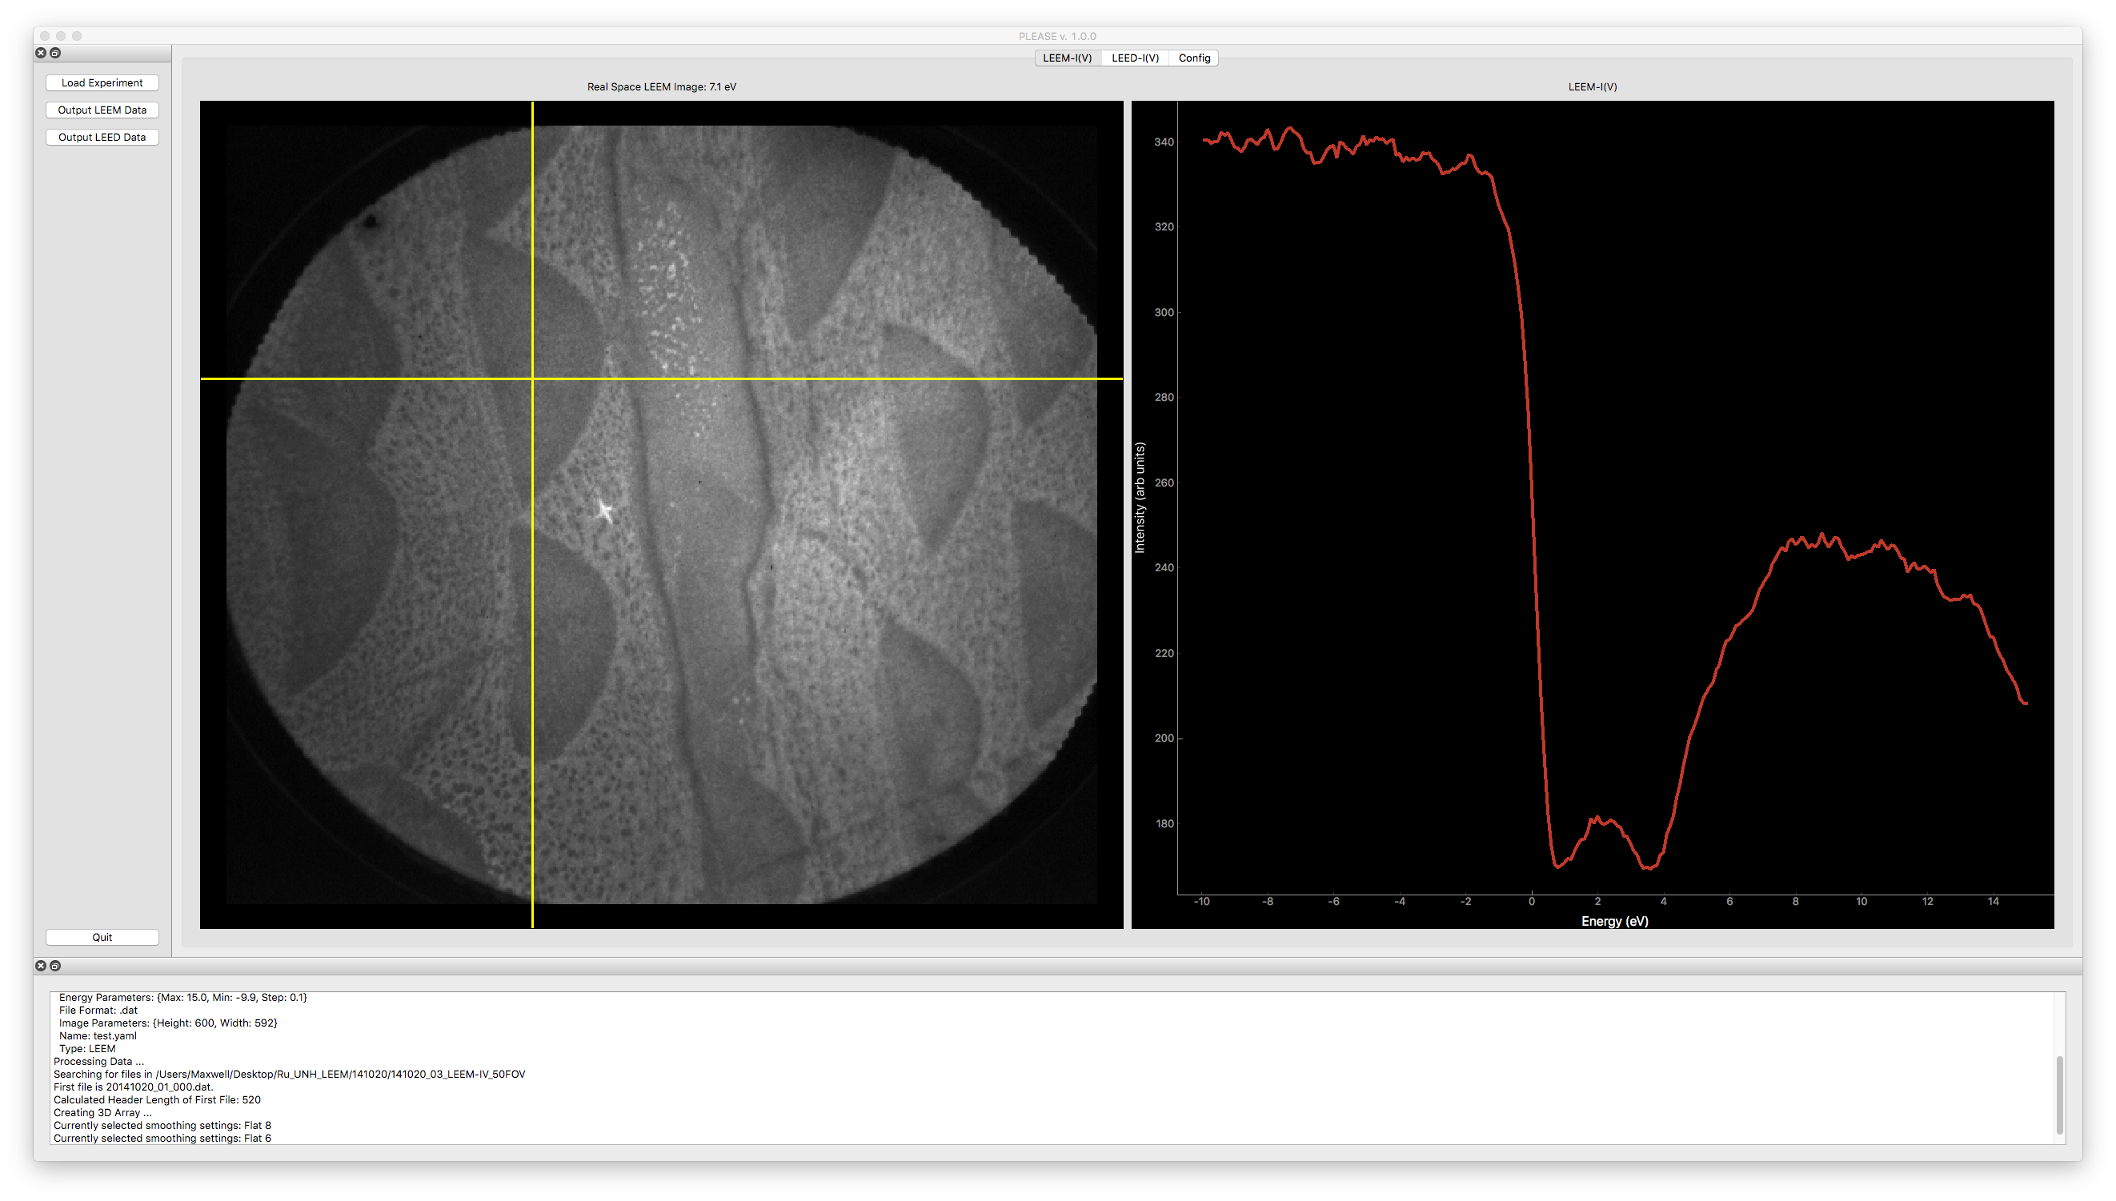
\includegraphics[scale=0.45]{figs/LEEM-IV150.png}
    \caption{50 $\mu$m field of view bright field LEEM image of graphene islands (dark areas) atop a ruthenium substrate (light). Image collected with incident electron energy of 7.1 eV. The \textit{I(V)} curve from an area on a graphene island marked by the yellow crosshair is plotted to the right.}
    \label{fig:please1}
\end{figure}

For LEED-\textit{I(V)} data, the extraction process is slightly different. Rather than extracting an \textit{I(V)} curve from a single pixel, the intensity of an entire diffracted electron beam spot must be summed and averaged then plotted against the incident electron energy. The size of the integration window for electron beam selection is a user configurable setting available in the CONFIG tab of the main PLEASE UI. Electron beams can be selected by left-clicking in the left hand image panel. A colored square window will be drawn centered on the user click location. \textit{I(V)} curves from up to ten selected areas can be extracted and plotted by choosing ``Extract-I(V)" from the LEED menu. The \textit{I(V)} curves will be plotted on the right hand panel and color coded to match the user selections. Figure \ref{fig:please2} demonstrates the extraction of multiple \textit{I(V)} curves from a LEED-\textit{I(V)} data set.


\begin{figure}
    \centering
        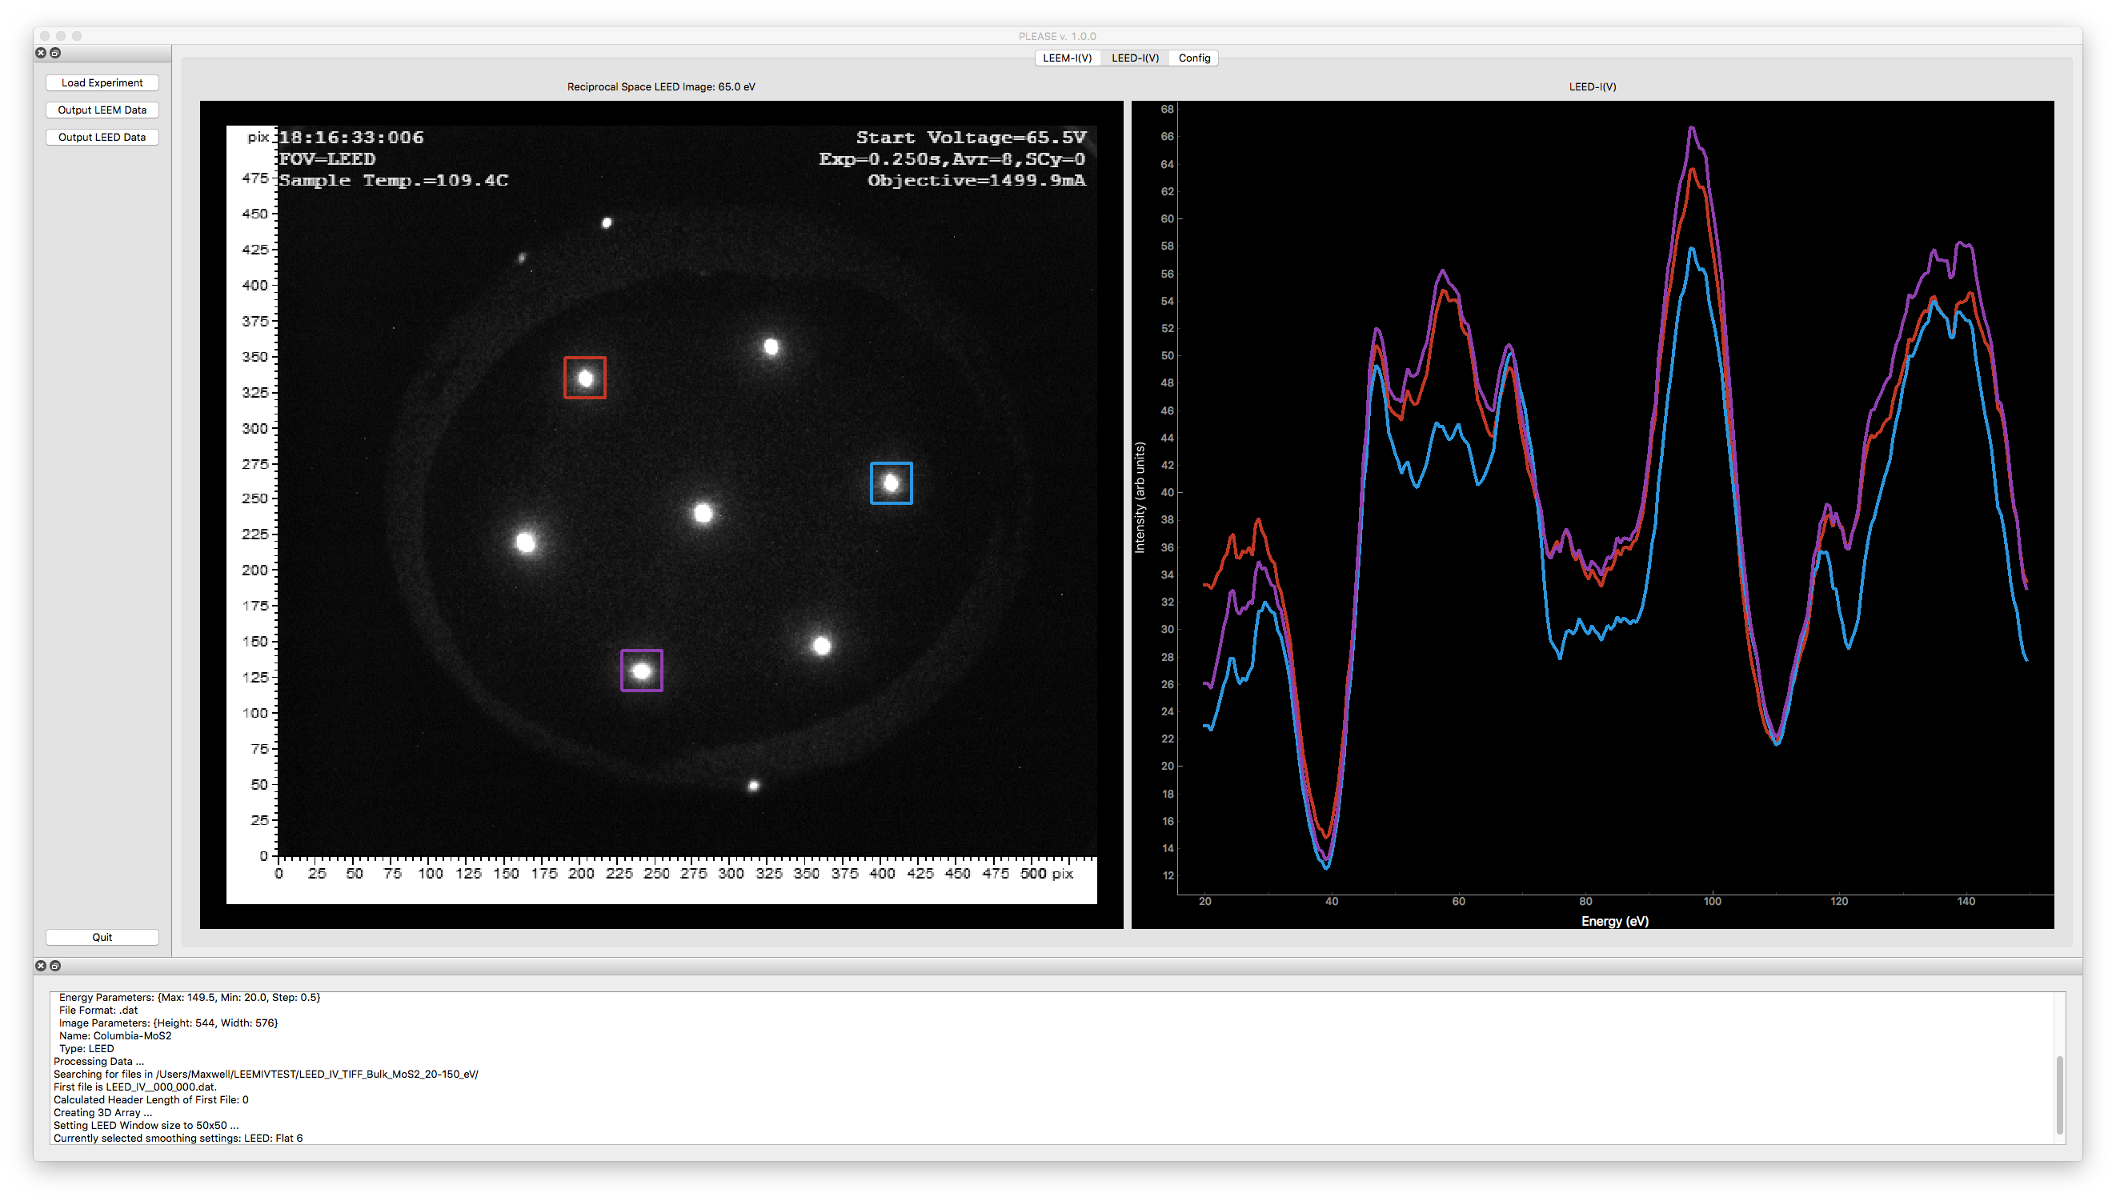
\includegraphics[scale=0.45]{figs/PLEASE-LEED-IV150.png}
    \caption{Reciprocal space image of MoS2 showing the diffraction pattern at a fixed energy alongside \textit{I(V)} curves from multiple symmetric diffraction beams using a 50 pixel x 50 pixel integration window.}
\label{fig:please2}
\end{figure}

\subsection{I(V) Output}
When \textit{I(V)} data has been extracted for LEEM or LEED data sets, the extracted curves can be output to a columnar tab-delimited text file. This is useful for recreating plots outside of the PLEASE GUI, formatting the \textit{I(V)} plots for publication, or a variety of post-processing techniques such as filtering to remove instrumental noise and noise from local inelastic electron scattering. \textit{I(V)} curves from multiple user selections will be output to separate text files. All I/O happens in a separate thread from the main UI thread, thus the UI will remain functional during the process of file writing.

\subsection{Standardized format for File Input}
In order to make PLEASE accessible for a wide range of users, multiple file formats are supported. To streamline the process of loading data for an experiment, I have created a standardized meta-data format for creating experiment configuration files using the YAML file format. These files tell PLEASE the correct parameters needed to load the data files for a given experiment. The necessary information for loading data is as follows:

\begin{itemize}
\item Path to data files
\item Experiment type (LEEM or LEED)
\item Image Parameters
    \begin{itemize}
       \item Image width in pixels
       \item Image height in pixels
       \item (optional) Image Bit Depth (8bit or 16bit) Required for loading raw data; no support for higher bit depth images
       \item (optional) Image Byte Order (Little Endian or Big Endian) Required for loading raw data
    \end{itemize}
\item Energy Parameters
     \begin{itemize}
       \item Starting energy in eV
       \item Final energy in eV
       \item Step energy in eV
     \end{itemize}
\end{itemize}

To provide convenience for the creation of YAML configuration files, a method is provide in the PLEASE GUI to create a new configuration file. From the File menu, selecting "Generate Experiment Config File" will open a dialog with input forms for all the required information listed above. File paths can be selected by clicking the corresponding button and navigating the dialog that appears. The information input by the user will be checked for validity before saving the file.

\subsection{Data Smoothing}
The raw data output from the LEEM instrument CCD will likely contain some level of instrumental noise resulting from the CCD itself as well as the micro-channel plate or similar technology used in the imaging column. As a result, there may be unwanted noise in the extracted \textit{I(V)} curves. To mitigate help mitigate this, the PLEASE software provides an easy to use data smoothing algorithm. \textit{I(V)} curves can be smoothed before plotting or writing to disk with a user configurable smoothing function. The smoothing is achieved by calculating the one-dimensional convolution of the intensity data from the \textit{I(V)} curve with a predefined window function. The window function and window length are user configurable options. The available windows are: Flat (Boxcar/Sliding Average), Bartlett, Blackman, Hanning, and Hamming. Boundary effects are minimized by extending the convolution region by introducing reflected copies of the signal at either end with length equal to the selected window length \cite{scipy-cookbook}.

\subsection{LEED Background Analysis Automation}
When analyzing LEED-\textit{I(V)} beams, there may be significant contribution to the observed \textit{I(V)} curve from the local background of inelastically scattered electrons. Thus, to improve the quality of the extracted \textit{I(V)} curve, it may be necessary to subtract an average background intensity obtained from the local vicinity of the selected electron beam. PLEASE provides an automated method for selecting local background curves from an electron beam. Once an electron beam has been selected, choosing "Auto Background Selection" from the LEED menu will generate six selection areas spread in a circle around the initial selection. Extracting the \textit{I(V)} will then show the intensity of the initial selection as well as the six background selections. This data can be output to text where the background intensity can be averaged and subtracted from the main beam intensity via post-processing. Figure \ref{leed-autobackground} demonstrates the automatic background selection process. Here it should be noted that while this method is convenient, it will not work properly for every LEED data set. The background selection boxes are  spread uniformly around a circle surrounding the initial user selection and their size scales with the size of the initial user selection. For certain LEED data sets with very closely spaced diffraction spots, the automatically generated background selection may overlap with areas that should not be considered background. For these data sets, instead the user should default to manually selecting background areas.

While PLEASE provides an easy method for selecting and extracting the background \textit{I(V)} from a data set, the actual background subtraction is left to the user, given that there is not necessarily one correct subtraction method that works on all data sets. Using the PLEASE software package's ability to output \textit{I(V)} to tab-delimited text files, the background subtraction can be accomplished relatively easy using python. Appendix B demonstrates an example of performing a background subtraction using data extracted using PLEASE and output to text.

\begin{figure}
  \centering
    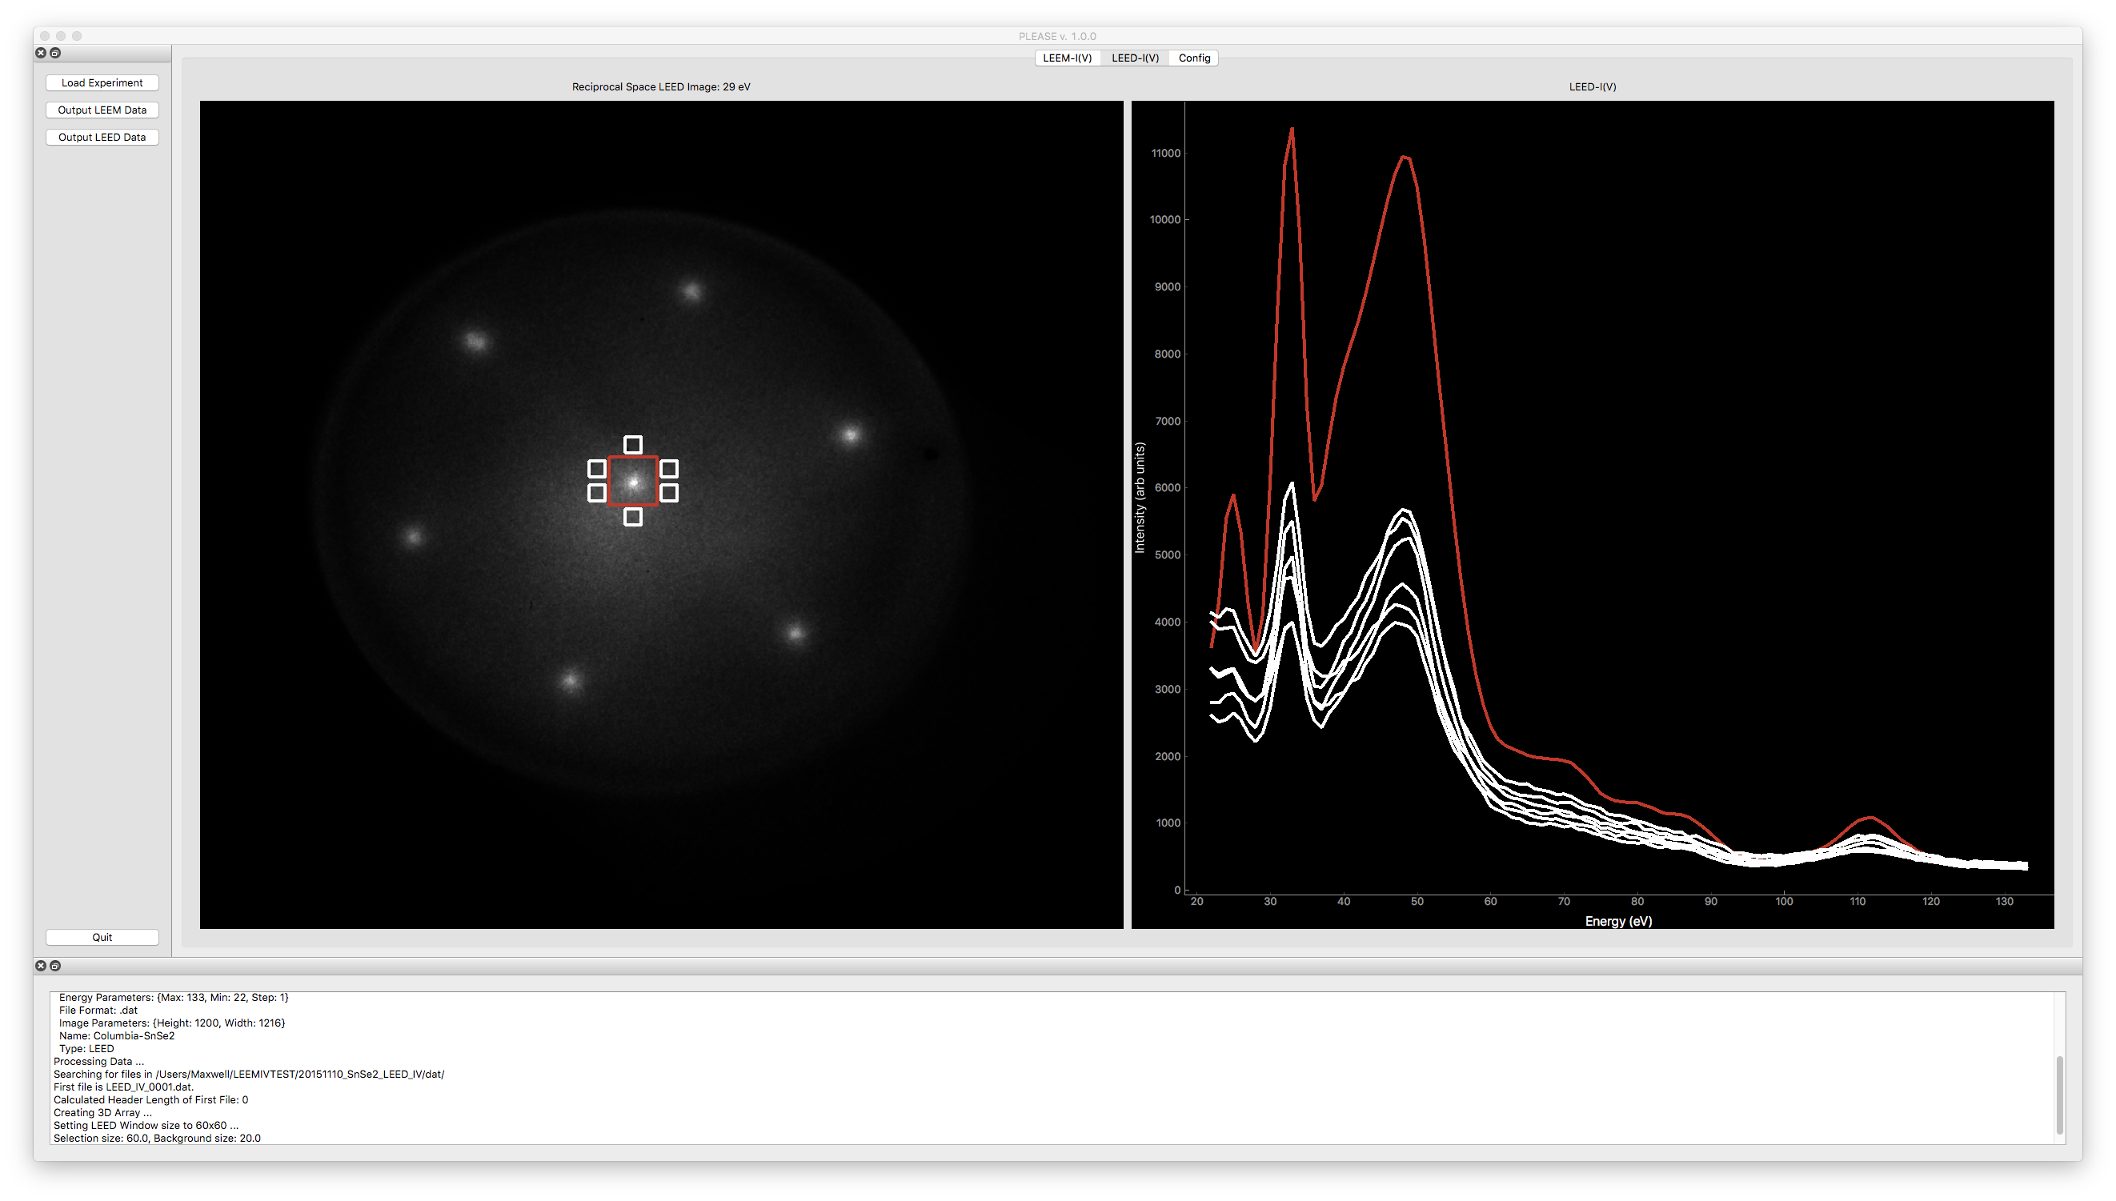
\includegraphics[scale=0.45]{./figs/LEED-AutoBackground150.png}
    \caption{
    LEED-\textit{I(V)} analysis of SnSe$_2$ demonstrating the automatic background analysis routine. The user selected electron beam \textit{I(V)} is plotted in red, the six background selections generated automatically have their corresponding \textit{I(V)} curves plotted in white.
    }
    \label{leed-autobackground}
\end{figure}


\section{Code}
The PLEASE software package is written entirely in python and designed to run on python versions 2.7 and 3.5+. It is highly recommended to use the latest version of python 3, however, python version 2.7 should still work fine. PLEASE does not support any python version less than 2.7 and no future support for legacy python versions is planned. For python 3, officially versions 3.5 and higher are supported, however, it may be possible to run on versions 3.3 or 3.4. These older versions of python 3 have not been tested and no future support is planned for these versions.


The source code for PLEASE can be found at \url{https://www.github.com/mgrady3/PLEASE} The main branch in the git repository should always be stable but may not contain the most up to date feature set. I maintain a number of branches for testing new features as they are added to the program but am not always as quick to merge working features into the main branch.
If in doubt, ask me about a given feature and I can provide the correct set of code to use.

The main github repository contains the source code, documentation, as well as a number of test data sets which can be used to ensure the software is functioning properly. Instructions for opening the test data are found within the test data directories in the main github repository.

More detailed instructions for installation and usage of the PLEASE software package can be found at the main github page listed above. It is recommended that you setup a python virtual environment for PLEASE so its dependencies do not conflict with other python software you may use. Instructions for how to do this are found in the Installation file in the main github repository.

Finally, given that the code is publicly available on Github, pull requests for new features and bug fixes are welcomed. Hopefully the code is structured in a way that will facilitate ease of use and modification. More information about contributing to the project can be found in the CONTRIBUTING file in the main github repository. In general the rule of thumb is to follow PEP8 guidelines when submitting code in a pull request.

\section{License}
\textbf{This software is released to the public under the GNU General Public License (GPL) included with the source code. The code may be freely used, modified, and distributed in accordance with this license. All required python libraries are subject to their own licensing terms and are not included under the license of this code.}

Please see the license file found within the main Github repository for full details concerning the licensing: \url{https://github.com/mgrady3/PLEASE/blob/master/LICENSE}

\section{Current and Future Work}
\begin{figure}
    \centering
    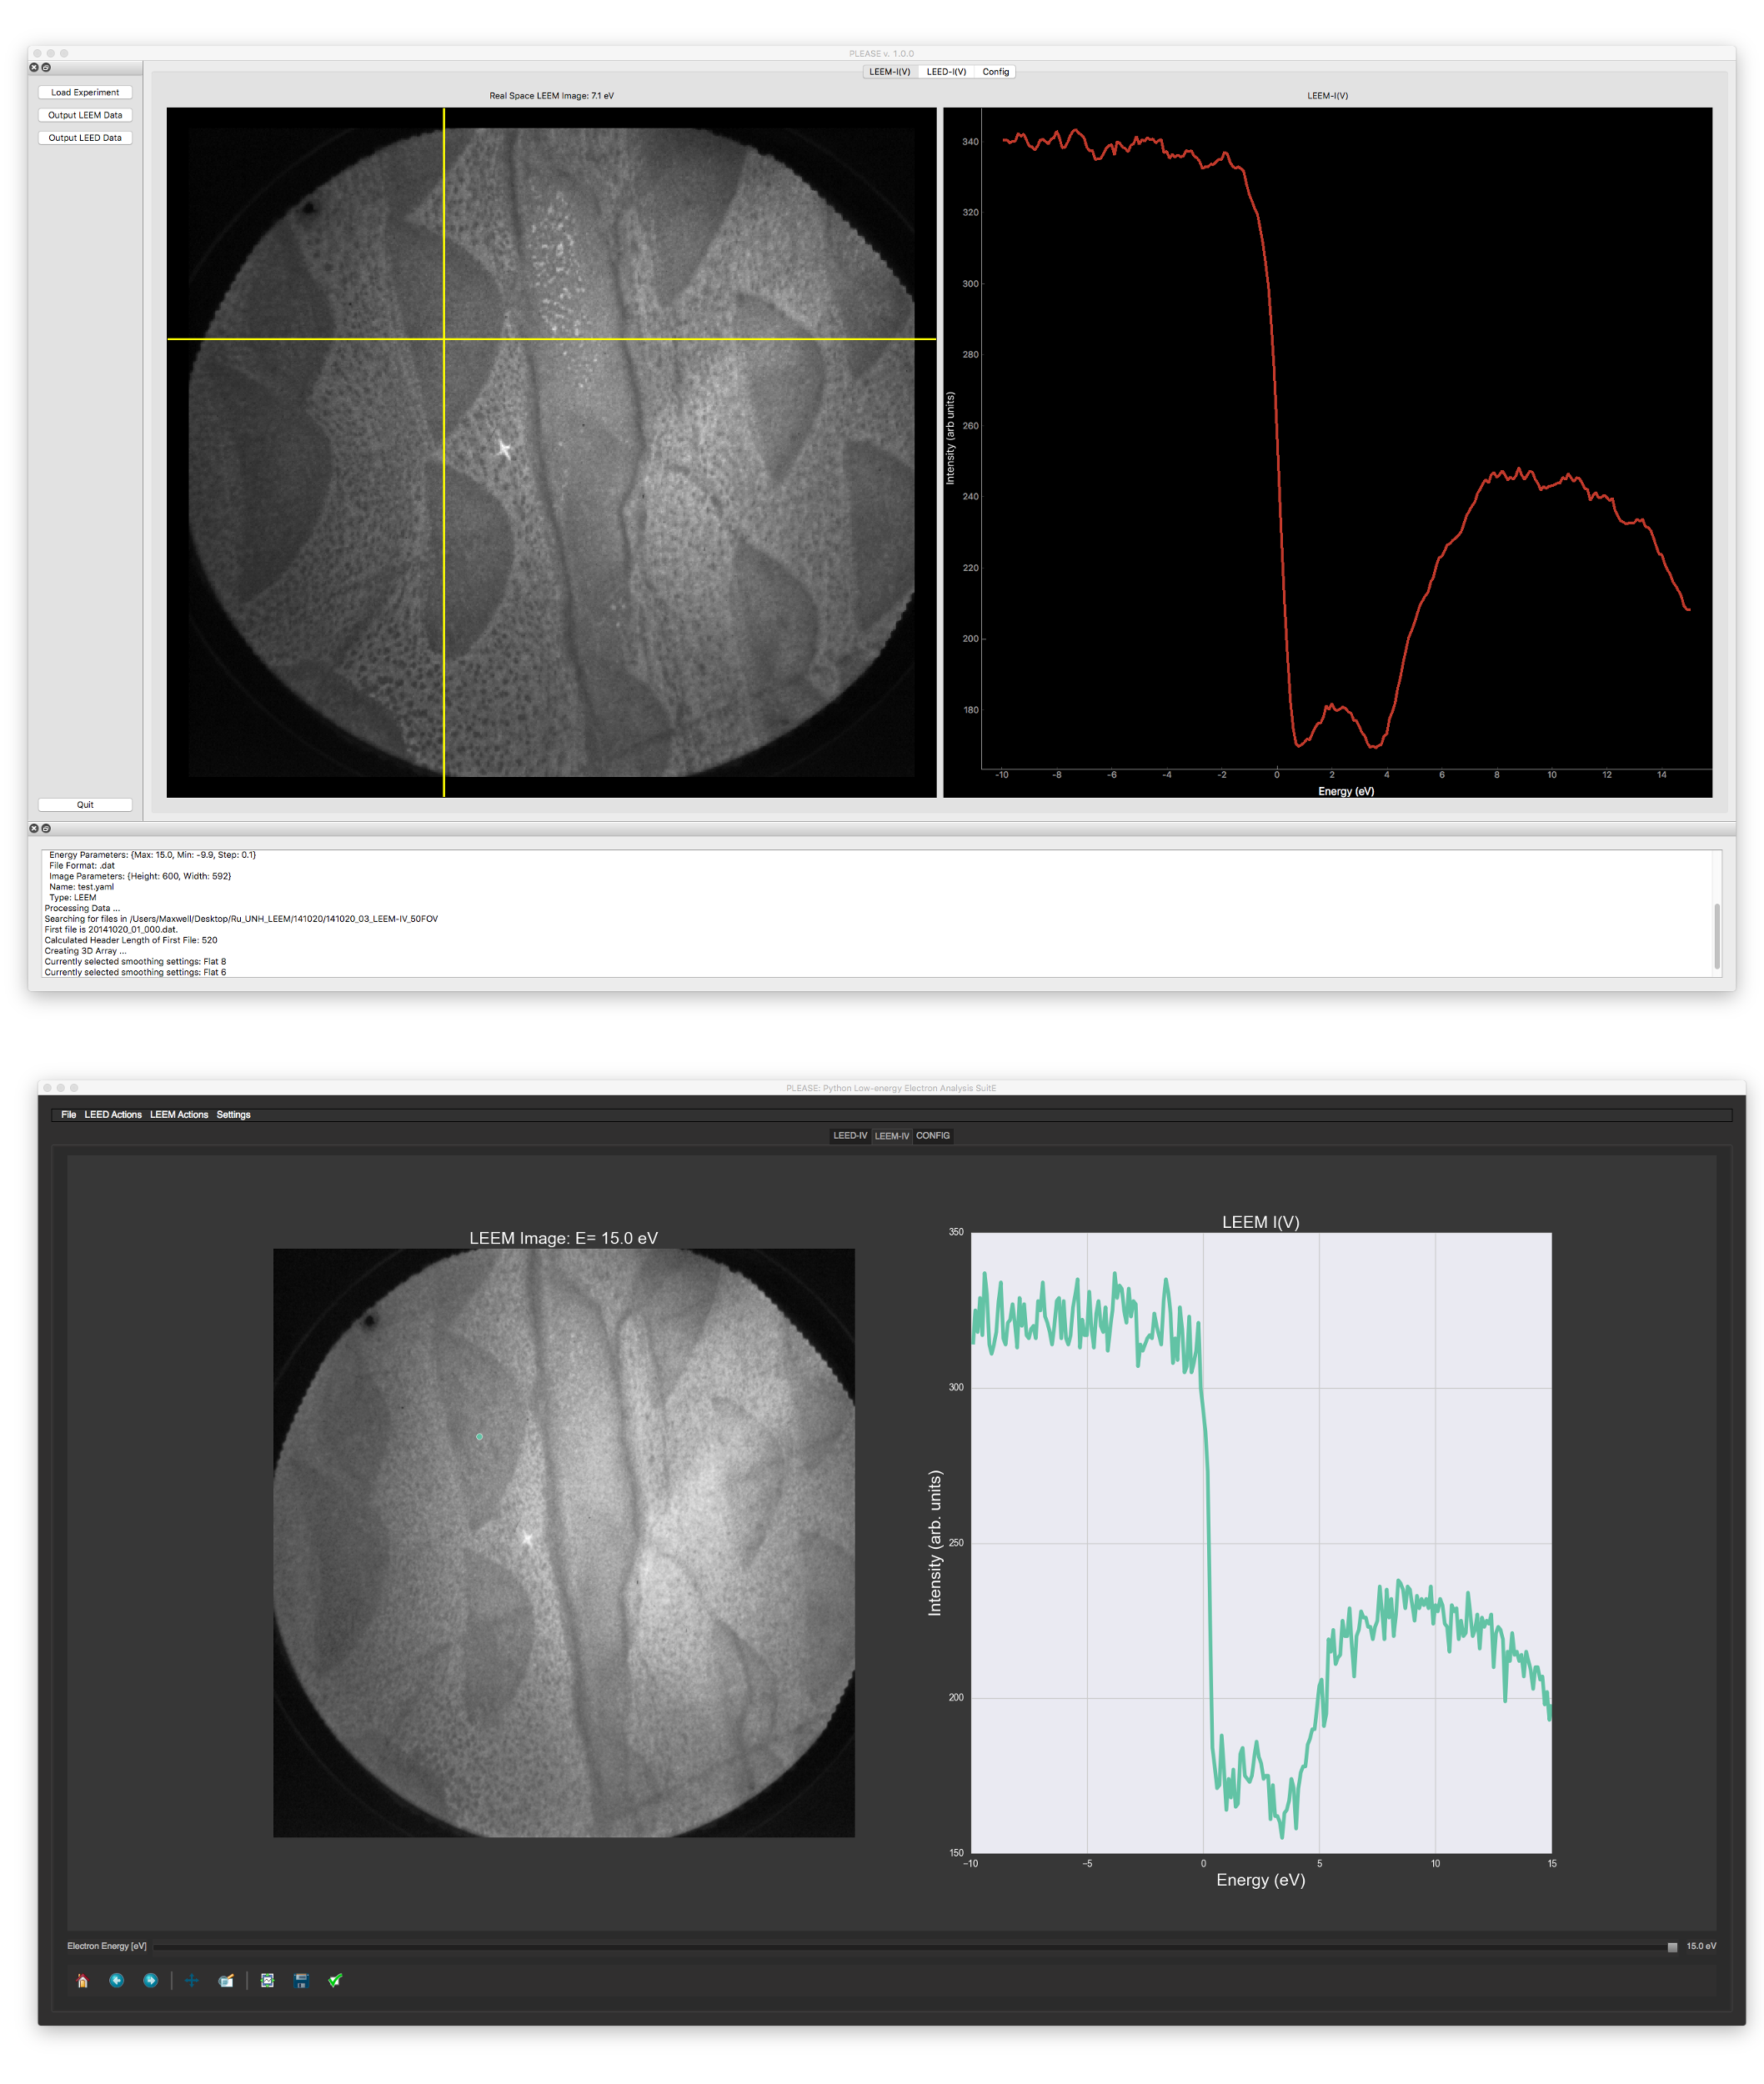
\includegraphics[scale=0.42]{./figs/PLEASE-old-new-150.png}
    \caption{Update to the design of PLEASE: The latest version of PLEASE, version 1.0.0, shown at the top, has been rewritten to leverage PyQtGraph in the backend for all image display and plotting. The old version, shown in the bottom, used Matplotlib figures embedded in a Qt widget.}
    \label{fig:PLEASE-Update}
\end{figure}
During its development, PLEASE has evolved from a command line script to process a single LEEM-\textit{I(V)} curve, to a full fledged GUI capable of analyzing numerous sets of both LEEM and LEED data. Over time the codebase has undergone two major rewrites. The most recent rewrite of the code completely changed the graphics library using for all data plotting to address a main concern from the old codebase. The legacy codebase relied on the python library Matplotlib to display all images and plots to the screen. While this worked fine for static plots, the library was ill-equipped to deal with rapid updates to the image display. For visualization of LEEM/LEED-\textit{I(V)} data sets, it is often useful to scan through the entire stack of images as a slideshow to check for things like beam motion in LEED images or contrast shifts in LEEM images. The Matplotlib event loop would often become bogged down when rapidly changing the image being currently displayed to the screen.

To address this issue the entirety of the PLEASE codebase was re-written to use PyQtGraph for all image and plot displays while still utilizing PyQt for the rest of the UI. In the backend, PyQtGraph uses the Qt QGraphicsView Framework (QGVF) for display purposes. The QGVF extends to the Model-View programing paradigm featured in numerous other languages and libraries, including Qt, to a collection of widgets centered on displaying images and graphs. This collection of widgets is highly optimized for real-time plotting and high fps animation and video.

Integrating PyQtGraph into the PLEASE software package not only solved the problem of lag when rapidly switching the displayed image but also allowed the LEEM portion of the program to perform extraction and plotting of \textit{I(V)} data in real-time. Rather than selecting a single spot on a LEEM image from the \textit{I(V)} data set to extract an \textit{I(V)} curve from, the program now automatically tracks the user mouse movement through the image, then extracts and plots the data from that location to the \textit{I(V)} plot. This all happens in near real-time with minimal lag, even when the user enables data smoothing for the \textit{I(V)} plots.

The current version of the software with the features detailed above integrated with PyQtGraph in the backend is stable, has been tested on all major operating systems, and can be downloaded from the Github master branch. Figure \ref{fig:PLEASE-Update} shows an example of the latest version of the PLEASE GUI in comparison to the previous version.

Each new set of experimental data analyzed with the PLEASE software package brings another opportunity to expand the functionality and enhance the user experience. There are a number of features currently being worked on for future releases of the software:

\subsection{Features under development}
The most complex of the new features provides a quality of use upgrade for extraction of LEED-\textit{I(V)} curves by implementing a beam tracking algorithm. Ideally, in a LEED-\textit{I(V)} data set acquired with a LEEM system, there should be little to no motion of the electron diffraction spots as the incident energy changes. However, due to circumstances often beyond control for a given experiment, there may be some shift in beam spot position as the incident energy changes. If the shift is relatively small then it may often be ignored so long as the extraction window size is large enough. However, to help with situations with larger beam motion, a method has been implemented to track the beam motion during the \textit{I(V)} extraction process and automatically shift the extraction window as needed.

Another feature of use for many LEEM and LEED experiments is to interpret a data set as a function of time rather than electron incident energy. For example, one can observe structural phase transitions by analyzing how a LEED pattern changes with temperature. By recording LEED images over time while simultaneously heating or cooling the sample, the pattern will change when the critical phase transition temperature has been passed. The data collected then is essentially \textit{I(t)} rather than \textit{I(V)}. Another example would be collecting real-time LEEM or PEEM images during the growth of a thin film by CVD, PVD, or MBE. Analyzing the LEEM or PEEM time series images shows how electron reflectivity or photoemission evolves over time during the growth process. To implement the ability to analyze time series data, a small addition of two parameters to the YAML meta-data configuration format has been indicates to the PLEASE software package that it should load the data as a time series set instead of an \textit{I(V)} data set. This has been implemented in a development branch and after some further testing will be ready to merge into the master branch as a main feature.

To complement time-series analysis, an additional feature being explored is the ability to output movies from the data images. The python package, MoviePy, makes this a relatively straightforward process, however, it also adds additional dependencies on the underlying FFMPEG engine in order to properly encode the files as videos. Initial work has been done as proof of concept that the movie file generation should work. What remains to be done is test the functionality on all major OS platforms, wrap the function into a GUI operation, and finally likely implement some method of allowing the main program to run without this feature simply disabled if the user does not have the proper dependencies for MoviePy to run. The last step may not be required depending on the outcome of testing the MoviePy library on alternate operating systems. If the installation of this library doesn't pose a problem on most operating systems, then it will be included as a full dependency of the PLEASE software package.

\subsection{Planned features not currently under development}
The final major feature being worked on would be a major overhaul or addition to the current method for loading data via the customized meta-data configuration files stored as YAML documents. The current method works well but can be somewhat cumbersome if a user has a very large number of experiments they currently analyze. Currently all of the burden is on the user to keep their experimental data organized in some fashion and the YAML files for each experiment up to date with the appropriate parameters. One possible method to help with the organizational problem would be to implement an experiment database and experiment parameter view to the main UI. When loading an experiment via a YAML file, an option would be provided to add this experiment to a database of experiments. At a later time, any previously opened experiment could be opened again by selecting the experiment from a TreeView widget allowing exploration (and possibly editing) of all the parameters from each experiment saved to the database. Likely the database could be implemented as a NOSQL variant using a simple key-value pair system for storing the experiments and their parameters as nested dictionary items. Having the database view be editable would give the user an easy way to change settings as needed or change the data path if the experiment data files are moved to a new location. Some initial work has been completed testing the viability of visualizing the experimental parameters in a TreeView widget, but no work as been started implementing the database backend to feed information to the view.

While there are a number of other minor features currently being worked on, the last to be mentioned here is a feature for static image analysis. Sometimes it may be useful to view images that are unrelated through time or incident energy. This may be a single image or a series of images. Currently the only way to do this is create a separate YAML configuration file for each image or series and spoof the ``Energy Settings'' section with arbitrary numbers only making sure that the total number of files is correct. In the future it would be convenient to have the ability to load static images without the need to create separate configuration files for each image. So far no work has been started on this feature though it is likely not a difficult feature to add.


% ------------------- %
